%
\chapter{Referencial Teórico}
\label{cap:ReferencialTeorico}

Neste capítulo são apresentados os conceitos que fundamentam o desenvolvimento deste trabalho. Na seção \ref{sec:AbandonoAnimaisDomesticos} são apresentadas as motivações para o abandono de animais domésticos; Na seção \ref{sec:AbandonoAnimaiPandemia}, o período pós pandêmico é considerado no estudo; Na seção \ref{sec:Informatização} é trabalhado o conceito de informatização dos processos; Na seção \ref{sec:SistemasWeb} é trabalhada a definição de Sistemas Web; Na seção \ref{sec:RedesSociais} é conceituado a respeito das Redes Sociais; Na seção \ref{sec:TecnologiasDeDesenvolvimento} são apresentadas as características das Tecnologias de Desenvolvimento utilizadas para construção deste trabalho.

\section{Abandono de Animais Domésticos}
\label{sec:AbandonoAnimaisDomesticos}
Os animais domesticados necessitam de carinho, proteção, afeto,  cuidados veterinários e uma boa alimentação durante todo o seu período de vida junto aos seus donos, porém a realidade é uma crescente parcela de animais que acabam por ser abandonados.

\cite{Schultz}, médica veterinária, em texto para o  Portal Nosso Mundo,  lista entre as motivações para o abandono de animais, o trabalho que eles demandam, gastos, necessidade de atenção, xixi pela casa, necessidade de adestramento e acompanhamento veterinário, seu crescimento além do previsto e a falta de estrutura física ou preparo psicológico dos tutores para manter o pet em sua casa. Ainda de acordo com ela, outra causa comum para a ocorrência de abandonos é a aquisição de animais em Pet Shops, que por muitas vezes é movida por um impulso momentâneo em adultos e crianças ao se deparar com um filhote bem cuidado e com preços atrativos. Animais vendidos em petshops por muitas vezes são resultado de criações de fundo de quintal, sem controle genético, desmamados e vendidos precocemente, o que compromete sua saúde, comportamento e capacidade de socialização.

\citeonline{Schultz} também adiciona entre as causas do abandono, a reprodução indiscriminada intermediada pelos guardiões destes animais, permitindo que os animais cruzem sem nenhum critério ou até mesmo permitindo a consanguinidade, gerando ninhadas com baixa variação genética e maior probabilidade de adquirirem problemas de saúde e desenvolvimento. 

\cite{Alvez} faz um levantamento das consequências decorrentes da presença de animais abandonados em locais públicos e sem supervisão, restrições e cuidados veterinários e com o agravante da presença destes em locais de saúde pública (devido às zoonoses), social (desconforto com relação ao comportamento animal), ecologia (em relação ao que se refere ao impacto ambiental) e econômico (custos com estratégias de controle populacional). 

Dentre as consequências do crescente número de animais nas ruas, é citado o envolvimento deste com problemas históricos de zoonoses, como a transmissão de raiva, leishmaniose, leptospirose, toxocaríase e outras doenças parasitárias, além dos casos de agressão humana aos humanos e a outros animais. Uma mordedura de um animal aumenta as chances da transmissão de zoonoses e compromete também a integridade física como a psicológica da vítima. \cite{Alvez}.

\newpage

\section{Abandono de Animais na Pandemia}
\label{sec:AbandonoAnimaiPandemia}
Em reportagem de Edison Veiga para a BBC News Brasil, é trazida a problemática da crescente onda de abandono de animais. \cite{Veiga}:

\begin{citacao}
"Seja pela crise, pelo medo de que cães e gatos transmitem coronavírus ou pela mudança de vida causada pela pandemia, mais donos de animais de estimação estão se desfazendo dos seus outrora melhores amigos".
\end{citacao}

Ao entrevistar o diretor da ONG Cão Sem Dono, Vicente Neto, foi levantada a informação de que houve um aumento de até 40\% na procura de novos donos para seus pets em comparação ao mesmo período do ano anterior, motivado pela crise do Coronavírus e por motivos relacionados, como a perda de empregos ou a mudança de residência.

O abandono de animais sempre atingiu em sua maioria os animais sem raça definida, mas hoje está se atingindo numerosamente também os animais ditos de raça, situação exposta na entrevista da fundadora da ONG Cão Sem Fome, \citeonline{Lombardi} à Edison Veiga:

\begin{citacao}
"E até mesmo cachorros de raça definida, que raramente apareciam nos abrigos, estão sendo deixados para trás por seus donos"\cite{Lombardi}.
\end{citacao}

O crescimento do número de animais abandonados não é um problema somente no Brasil, mas sim de âmbito mundial. Em reportagem de Flávia Duarte para CNN, em Londres, é mostrado que com a quarentena obrigando a população a ficar meses em casa, muitas pessoas acabaram por adotar animais por impulso, mas que com a reabertura de escritórios, lojas e restaurantes, estes animais vêm sendo abandonados, se tornando uma crise de aspecto mundial.

\begin{citacao}
"A maior organização de proteção animal da Inglaterra afirma que, à medida que os escritórios, lojas e restaurantes 	começaram a reabrir, os abrigos receberam uma enxurrada de animais abandonados. O ato é visto em vários países do mundo como crise canina" \cite{Duarte}.
\end{citacao}


\section{Informatização}
\label{sec:Informatização}
\citeonline{Planez} cita que a partir do século XXI, a popularização dos computadores e internet permitiram que os benefícios da informação chegassem à maioria das pessoas, o que causou uma revolução comportamental e de consumo, mudando o cenário econômico mundial e gerando uma nova economia baseada em redes de comunicação. \citeonline{Muller}, por sua vez, defende que estamos vivendo o ápice da influência tecnológica em nossas vidas e que esta influência traz impactos positivos e negativos, alterando os hábitos das crianças e adultos, sobretudo com a Internet, que trouxe comodidades, empregos, redes sociais e entretenimento. 

Os pontos de vista de Planez e Muller demonstram que a informatização dos processos têm impacto direto na sociedade, em seus hábitos, nas relações sociais, no trabalho,e está em constante expansão, abrangendo cada vez mais áreas de nossas vidas. As soluções computacionais se fazem presentes como ferramentas de trabalho, auxílio em estudo, momentos de lazer, compras, pagamentos, busca de relacionamentos e expansão dos métodos de comunicação para além da oralidade \cite{Muller}. 
De acordo com o site \citeonline{internetlivestats}, que faz um acompanhamento em tempo real da quantidade de usuários de internet e de Websites criados no mundo, hoje já são mais de 5.385.798.406 pessoas conectadas e mais de 1.892.144.189 Websites na rede. Em pesquisa divulgada pelo site da Empresa Brasil de Comunicação (\gls{EBC}), \citeonline{ebc}, em 2020 já havia mais de 134 milhões brasileiros acessando a internet. (Figura \ref{fig:Informatização}).

\begin{figure}[htb]
     \centering
     \FonteFig{\citeonline{internetlivestats}}
     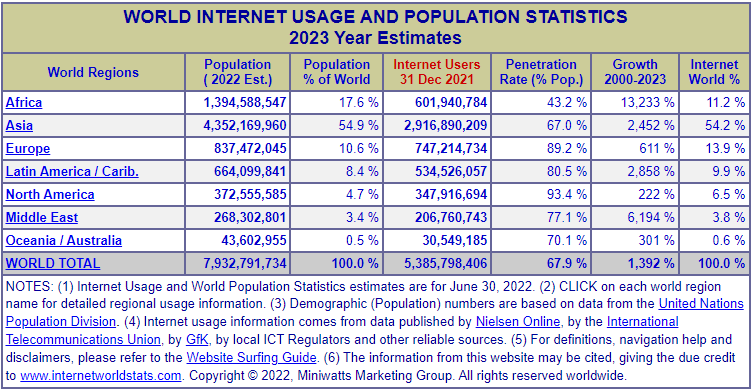
\includegraphics[width=14cm]{arquivos/Figuras/figura 01.png}
     \caption{World Internet Usage And Population Statics}
     \label{fig:Informatização}
\end{figure}


\newpage
\section{Sistemas Web}
\label{sec:SistemasWeb}
\citeonline{Noleto} define aplicação web como uma solução executada diretamente no browser e que por ser utilizada nos navegadores é de fácil acesso e uso pela maioria das pessoas. Ele também acrescenta que existe diferenciações importantes entre os sistemas web e os sistemas chamados de tradicionais, sendo que estes tidos como tradicionais necessitam de instalação na máquina do usuário e as informações disponíveis neles são padronizadas ou seja, iguais nas diferentes máquinas e em diferentes acessos, por sua vez, em sistemas web atuais, as informações são personalizadas e adaptadas de acordo com cada visitante.

Semelhante ao defendido por Noleto, \citeonline{Barros}, consultor do Núcleo de Tecnologia da Empresa Júnior de Engenharia e Arquitetura da USP São Carlos (\gls{EESC Jr}), interpreta que os sistemas web são sistemas dinâmicos, que permitem a criação de contas e fornecem experiências personalizadas aos seus usuários indo de acordo com as suas preferências e seus comportamentos, não dependendo da instalação de aplicações além de um navegador.

\section{Redes Sociais}
\label{sec:RedesSociais}
No artigo intitulado Redes sociais online: o que são as redes sociais e como se organizam?, da professora \citeonline{Luciana}, é exposta a seguinte definição para Redes Sociais: 

\begin{citacao}
"Entende-se, como Rede Social online, o ambiente digital organizado por meio de uma interface virtual própria (desenho/mapa de um conceito) que se organiza agregando perfis humanos que possuam afinidades, pensamentos e maneiras de expressão semelhantes e interesse sobre um tema comum".
\end{citacao}

Ainda neste artigo, \citeonline{Luciana} complementa o entendimento:
 
 \begin{citacao}
"[...]Rede social online como uma representação de relacionamentos afetivos e/ou profissionais entre indivíduos que se agrupam a partir de interesses mútuos e tecem redes informacionais por meio das trocas discursivas realizadas no ambiente virtual".
\end{citacao}

\section{Tecnologias de Desenvolvimento}
\label{sec:TecnologiasDeDesenvolvimento}
Para o desenvolvimento do MeuPetAqui, foram utilizadas uma variedade de tecnologias, incluindo \gls{HTML}, \gls{CSS}, JavaScript, \gls{PHP}, Laravel, ReactJS e MariaDB. Além disso, foi empregado bibliotecas relacionadas a algumas dessas tecnologias para facilitar o desenvolvimento e aproveitar ferramentas já desenvolvidas pela comunidade de programadores. 

\subsection{HTML}
HTML, CSS e JavaScript são frequentemente referidos como a "santíssima trindade" dos desenvolvedores front-end, pois formam a base de toda aplicação desse tipo. Em 1991, Tim Berners-Lee projetou o HTML como uma linguagem de marcação para permitir o compartilhamento prático de documentos. Inicialmente, o objetivo era interligar pesquisas científicas, mas com a criação da World Wide Web (\gls{WWW}), o uso da linguagem se tornou amplo e universal \citeonline{Ballerini}.

O HTML é uma linguagem de marcação que se enquadra na categoria "Tag Language". Nessa linguagem, os comandos são escritos em marcações chamadas de tags, as quais geralmente são apresentadas em pares. A tag inicial delimita o início da formatação do texto e a tag de fechamento delimita o final. A estrutura de um documento HTML é iniciada com a tag <HTML> e é dividida em duas partes principais: o cabeçalho e o corpo do programa. Essas partes são representadas pelas tags <HEAD> e <BODY>, respectivamente. É importante destacar que outras tags podem ser utilizadas no cabeçalho e no corpo do código. \cite[p. 6-7]{Pedroso}.

Com o crescente uso do HTML, os desenvolvedores se interessaram cada vez mais por tornar suas páginas mais atraentes e personalizadas. No entanto, a estilização do HTML diretamente em seus arquivos compromete a estruturação e compreensão do código. Para solucionar esse problema, em 1995 foi criado o CSS, possibilitando o tratamento da estética das páginas de forma separada da estrutura \cite{Ballerini}.

\subsection{CSS}
De acordo com a \citeonline{MDNWebDocs}, em sua página oficial da Mozilla para desenvolvimento de padrões web e projetos Mozilla, o CSS (Cascading Style Sheets) é responsável por dar estilo e aparência às páginas da web. Embora não seja uma linguagem de programação, assim como o HTML, o CSS também não é uma linguagem de marcação. Em vez disso, é uma linguagem de folhas de estilos e para ser utilizada, deve ser aplicada a um documento HTML para ser utilizada.

\subsection{JavaScript}
O JavaScript, de acordo com \citeonline{Ballerini}, é uma linguagem resultante da competição das gigantes Microsoft e Netscape, ambas empresas desenvolveram linguagens para implementarem em seus servidores e posteriormente passaram a rodar diretamente em seus navegadores, sendo o JScript da Microsoft e o Javascript da Netscape. No entanto, cada linguagem era compatível somente com o respectivo navegador da sua empresa,  Por isso, houve a necessidade de padronização destas linguagens, assim a Netscape enviou dados da sua linguagem para a \gls{ECMA}, permitindo a sua incorporação em mais navegadores.

\newpage
\subsection{React}
ReactJS é uma biblioteca JavaScript para a criação de interfaces de usuário. Foi criada pelo Facebook em 2011 com objetivo de otimizar e simplificar a atualização e sincronização do feed de notícias da rede social, chat, status entre outros recursos da rede social. Além disso, o ReactJs facilita a conexão entre HTML, CSS, JavaScript e todos componentes da página \cite{Roveda}.

De acordo com \citeonline{Prata}, o uso da biblioteca é uma ótima opção para a criação das interfaces de usuário (\gls{UI}’s) devido à sua capacidade de simplificar o processo de desenvolvimento e por proporcionar uma melhor experiência de uso ao usuário final.  Isso se dá pelo uso da programação declarativa, o que muda o foco do desenvolvimento para o "O que", ao em vez do "Como" \cite{Prata}.

\begin{citacao}
"Precisamos nos preocupar mais com 'O que' e menos com o 'Como'. Em outras palavras, precisamos simplesmente 'falar' para o React: 'Dado o estado X na minha aplicação, apresente a UI desta forma para o usuário'”\cite{Prata}.
\end{citacao}.

Outra qualidade do ReactJS apontada por ele, é a biblioteca ser baseada em componentes, o que permite criar componentes reutilizáveis para construir interfaces. É possível separar a interface em partes independentes e reutilizáveis, tornando o ReactJS uma das principais bibliotecas de front-end do mercado \cite{Prata}.

\citeonline{Guedes2} destaca que o ReactJS é uma das ferramentas mais utilizadas no mercado, tanto em termos de número de pessoas envolvidas quanto de empresas que a utilizam. Grandes empresas, como Netflix, Airbnb, American Express, Facebook, WhatsApp, eBay e Instagram, usam o ReactJS em seus sistemas. Segundo Andrei L (2021), o ReactJS é fácil de usar, escrever e apresenta um bom desempenho com o Virtual \gls{DOM}, além de ser amigável ao ao Search Engine Optimization (\gls{SEO}).

\subsection{PHP}
De acordo com \citeonline{Estrella}, o PHP é uma linguagem de script do tipo server-side, ou seja tem seu foco na implementação ao lado do servidor ou como é popularmente categorizada, uma linguagem de back-end. Ele também o descreve como uma linguagem versátil e capaz de gerar conteúdos dinâmicos para um site, sendo utilizada hoje por cerca de 79\% dos sites, em plataformas de ecommerce, blogs, redes sociais dentre outras aplicações.

O PHP foi criado em 1995 pelo programador cadadense Rasmus Lerdorf, sendo a sua sigla um acrônimo para Hypertext Preprocessor. Para \citeonline{Melophp}. A linguagem pode ser considerada fácil de se aprender e conta com recursos avançados e bom desempenho. Segundo informações do site \citeonline{W3techs}, que faz pesquisas de acompanhamento a respeito das diversas tecnologias de desenvolvimento, de acordo com os dados de 1 de abril de 2023, 77.5\% dos Websites existentes hoje, utilizam em sua programação o PHP, sendo desta porcentagem, 66.1\% a versão 7 da linguagem, 21.2\% a versão 5, 12.5\% a 8 e 0.2\% a 4. Tabela de dados na Figura \ref{fig:PHP}.

\begin{figure}[htb]
     \centering
     \FonteFig{ \citeonline{W3techs}}
     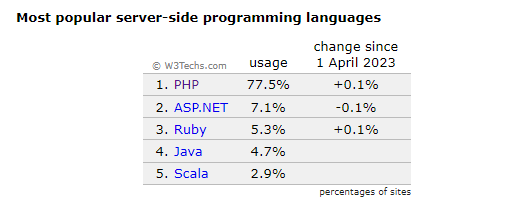
\includegraphics[width=14cm]{arquivos/Figuras/usodophp.png}
     \caption{Most popular server-side programming languages}
     \label{fig:PHP}
\end{figure}

\newpage
\subsection{Laravel}
O Laravel, criado por Taylor Otwell, é um dos frameworks mais populares atualmente para o desenvolvimento web, estando na versão 10. O seu uso da arquitetura \gls{MVC} (Modelo, Visão e Controle) ajuda no desenvolvimento de aplicações, simplificando processos, melhorando a segurança e a performance, além de deixar o código mais limpo e simples, incentivando boas práticas de programação e seguindo o padrão PSR-2 para guiar no estilo de escrita de código \cite{Weldell}.

De acordo com Rossi (2020), o Laravel facilita o trabalho com bancos de dados através do Eloquent \gls{ORM}, que traz várias funcionalidades para inserção, atualização, busca e exclusão de registros. Com a sua implementação, o framework torna o trabalho com o banco de dados mais fácil e simples, além de proporcionar uma conexão facilitada com o banco de dados \cite{Weldell}.

Existem diversos motivos para escolher o Laravel como framework de desenvolvimento de aplicações web. O fato de ser de código aberto e gratuito é uma grande vantagem, assim como a facilidade de escalabilidade do sistema, permitindo a adição de novas funcionalidades e recursos de forma rápida e eficiente, o que é importante em projetos de longo prazo que precisam se adaptar a mudanças de requisitos e necessidades dos usuários. O Laravel também possui uma documentação bem estruturada e organizada, facilitando o processo de aprendizado. Além disso, a sua popularidade é um fator importante, com uma grande comunidade de usuários e desenvolvedores ativos em fóruns e comunidades, dispostos a colaborar com a resolução de problemas \cite{MeloLaravel}.

Em artigo para a EDUCBA, uma plataforma de aprendizagem online da Àsia, \citeonline{SwatiTawde} enumera os principais recursos do Laravel, sendo eles:
\begin{itemize}
\item {\bf Dependency Management:} É um meio de injetar ou remover recursos codificados em um sistema, permitindo a gerência de dependências de forma eficiente e organizada.
\item {\bf  Modularity:} Permite a separação ou recombinação de partes da aplicação em vários componentes, que trabalham em conjunto para o funcionamento do sistema, tornando-o mais escalável, flexível e fácil de manter.

\newpage
\item {\bf  Authentication:} É um recurso essencial em todos os aplicativos web e, no Laravel, pode ser implementado com facilidade e poucos comandos, garantindo a segurança e a proteção de dados sensíveis.

\item {\bf  Caching:} Funciona como um meio de armazenamento temporário de dados, permitindo acesso rápido quando necessário, melhorando a eficiência da aplicação e aumentando a sua performance.

\item {\bf  Routing:} Permite agrupar, nomear, filtrar e conectar as informações do modelo aos caminhos, criando rotas flexíveis e controladas para se criar URLs amigáveis aos mecanismos de busca.

\item {\bf  Security:} Utilizando BCrypt, o Laravel salva as senhas como hash, tornando-as mais seguras. Além disso, oferece segurança contra ataques de injeção de SQL e controle das entradas do usuário, evitando a entrada de tags de script maliciosas.

\item {\bf  Migration System:} É usado para construção de bancos de dados, gerando bases, tabelas e índices, permitindo a repetição do processo de migração sempre que necessário fazer uma alteração no arranjo do banco de dados.

\item {\bf  Artisan:} Também chamado de Artesão, é uma ferramenta com dezenas de comandos pré-construídos que executam tarefas de rotina, evitando repetições de tarefas e facilitando o desenvolvimento.

\item {\bf Database Query Builder:} Oferece facilidade em criar solicitações ao banco de dados, incluindo funções que auxiliam a filtrar dados e fazer consultas complexas, simplificando a escrita de consultas ao banco.

% \newpage
\item {\bf RestFul Controllers:} Permite a separação de requisições Get ou Post, permitindo a construção de controladores de recursos fáceis de usar para construir o CRUD(Create, Read, Update, Delete), sendo possível conectar o controlador de recursos ao caminho para atender automaticamente todos os caminhos do CRUD.
\end{itemize}

% \begin{figure}[htb]
%      \centering
%      \FonteFig{educba.com (2023)}
%      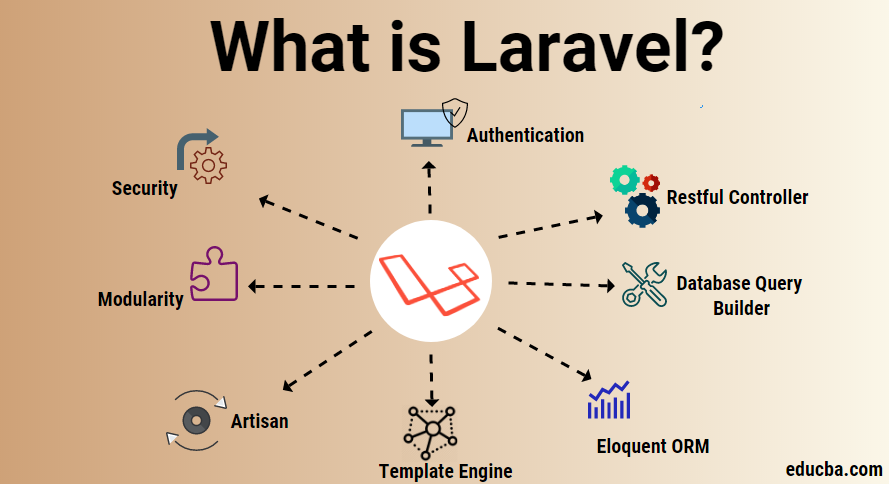
\includegraphics[width=14cm]{arquivos/Figuras/What-is-Laravel.png}
%      \caption{What is Laravel?}
%      \label{fig:Laravel}
% \end{figure}
\newpage
%%%%%%%%%%%%%%%%%%%%%%%%%%%%%%%%%%%%%%%%%%%%%%%%%%%%%%%%%%%%%%%%%%%%%%%%%%%%%%%%%%
%%%%%%%%%%%%%%%%%%%%%%%%%%%%%%%%%%%%%%%%%%%%%%%%%%%%%%%%%%%%%%%%%%%%%%%%%%%%%%%%%%
%% REMOVIDO POR NÃO ACHAR LINK DA FONTE
% \section{API}
% As APIs intermediam a comunicação entre dois sistemas ou plataformas, possibilitando a troca de dados entre sistemas distintos, integração e funcionamento. As APIs podem ser privadas ou públicas, sendo que o que difere delas, é que os dados das privadas são fornecidos somente para as organizações as quais as desenvolveram. (Brandão, 2020).

% A API do MeuPetAqui possui algumas de suas rotas com acesso público. Assim, desenvolvedores, empresas e interessados podem aproveitar os registros de pets perdidos, encontrados, para adoção ou que passaram por tratamentos registrados na rede social, estimulando o surgimento de novas aplicações que possam se integrar ao sistema ou contribuir para a causa animal.
\newpage
\subsection{Banco de Dados}
Banco de Dados é uma coleção organizada de informações/dados armazenados em um sistema de computador, divididos em tipos diferentes, como Relacionais, Orientados a Objetos, Distribuídos, Data Warehouses, NoSql, Gráficos ou \gls{OLTP}. O conceito de banco de dados pode ser simplificado em um agrupamento de dados do mesmo assunto, gerenciado por um serviço \gls{SGBD} \cite{Andrade}.

O planejamento do banco de dados deve garantir organização das informações, boa performance e facilitar manutenções e upgrades. Durante a construção do modelo conceitual é importante a participação dos usuários e a validação por eles. Esse processo se divide em duas fases, a modelagem conceitual e o projeto lógico \cite{RicardoBD}.

Inicialmente, o mercado de Banco de Dados era dominado pela Microsoft e Oracle, até que em 1995 surgiu o MySQL, ganhando espaço pela praticidade na gestão de dados e por ser uma solução gratuita. Entretanto, o MySQL foi vendido para a Sun Microsystem e depois para a Oracle, acarretando mudanças, como a descontinuidade da gratuidade do uso. Nesse cenário, surgiu o MariaDB, criado pelos mesmos desenvolvedores do MySQL e sendo um "fork" do projeto. O MariaDB, projeto de Michael Widenius, foi lançado em 2009 e é mantido pela MariaDB Foundation, além de ser disponibilizado gratuitamente para fins comerciais ou não \cite{Rafael}.

O MariaDB vem se mantendo constantemente atualizado, quanto a seu desempenho, funcionalidade e segurança, sendo uma ótima opção para pequenos e grandes projetos.

\newpage
\chapter{Trabalhos Correlatos}
Neste capítulo são apresentados sistemas correlacionados com o MeuPetAqui, caracterizando-se como redes sociais voltadas para os animais de estimação e o quadro comparativo entre as funções disponíveis entre eles.

\section{Flockr}
De acordo com informações presentes em seu site \citeonline{FLOCKR}, acessado em 01 de maio de 2023, Flockr se trata de um conjunto de três serviços de um sistema relacionado aos animais de estimação e assinatura de plano de saúde, sendo que os segmentos que são abarcados pelo sistema são: 

\begin{itemize}
\item {\bf Rede Social}: O dono do pet cria um perfil de usuário que é destinado ao seu pet de forma gratuita, nesta rede social é possível interagir com outros usuários,  postar fotos, comentar e dar likes em postagens. O Flockr possui um registro de passeios, em que o dono do pet pode compartilhar o tempo e distância do passeio com o seu pet entre os amigos da rede.

\newpage
\item {\bf Carteira de saúde}: A carteira de saúde do sistema tem funcionalidades de organização da agenda do animal, registrando e monitorando datas de vacinação, vermífugos, anti pulgas e outros medicamentos, visitas ao pet shop para banhos. Com a carteira de saúde também é possível fazer o acompanhamento da variação de peso, doenças e alergias que o pet adquiriu durante a sua vida. A carteira de saúde faz parte da rede social, sendo gratuita em suas funcionalidades.

\item {\bf Flockr Premium}: Flockr Premium adiciona funcionalidades para a carteira de saúde, com a assinatura do serviço premium o usuário poderá fazer a gestão dos gastos de cada segmento de serviço disponível na carteira de saúde, além de adicionar verificação ao perfil do pet, adição de molduras em imagens, efetuar perguntas para veterinários parceiros da aplicação, que são respondidas em posts de um blog associado. A assinatura do serviço premium é de cobrança mensal, custando no momento da pesquisa, maio de 2023, R\$49,90.
\end{itemize}

As funções como carteira de vacinação digital, histórico de peso, lembretes de medicamentos, agendamento de consultas, registro de passeios dentre outros fazem parte do plano premium do serviço. (Figura \ref{fig:Flockr}).


\begin{figure}[htb]
     \centering
     \FonteFig{Flockr/Reprodução}
     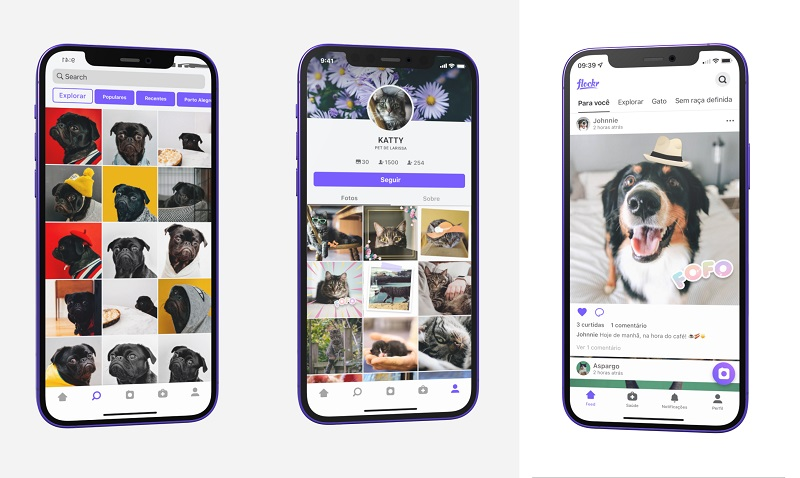
\includegraphics[width=14cm]{arquivos/Figuras/florckr.jpg}
     \caption{Interface Aplicativo Flockr}
     \label{fig:Flockr}
\end{figure}

Existem diferenças notáveis entre os serviços oferecidos pelo sistema Flockr e pelo MeuPetAqui. Uma distinção significativa é que o Flockr é uma aplicação que disponibiliza parte dos seus serviços mediante pagamento, o que pode afastar uma parcela de potenciais usuários em comparação com o MeuPetAqui, que deve oferecer os seus serviços de forma gratuita. Além disso, uma funcionalidade importante que destaca as duas plataformas é a ausência de recursos de rastreamento de animais perdidos no Flockr, o que pode ser um aspecto a ser considerado pelos usuários que buscam uma opção que ofereça segurança e localização para seus animais de estimação.
\newpage


\section{Pet Ponto}
Com base em uma pesquisa realizada no site do \citeonline{PETPONTO}, acessada em 03 de maio de 2023, foi possível observar que a plataforma se divide em um sistema web e um aplicativo móvel. No site, as funções de cadastro permitem aos usuários realizar adoções ou informar o encontro de um pet, enquanto ONGs ou protetores podem cadastrar pets para adoção ou encontrados. Já o aplicativo Pet Ponto conta com um sistema de geolocalização para filtrar e recomendar pets disponíveis para adoção, apresentando os animais em ordem de proximidade ao usuário que deseja adotá-los.

O sistema Pet Ponto funciona como um catálogo de animais, permitindo que os usuários selecionem quais animais desejam visualizar por sexo, espécie, estado e cidade em que eles estão disponíveis. Até a data da pesquisa, em 03 de maio de 2023, o sistema só apresentava pets do Rio de Janeiro, São Paulo e Paraná, mas o objetivo da plataforma é alcançar uma abrangência nacional. (Figura \ref{fig:Pet Ponto}).

\begin{figure}[htb]
     \centering
     \FonteFig{Pet Ponto/Google Play}
     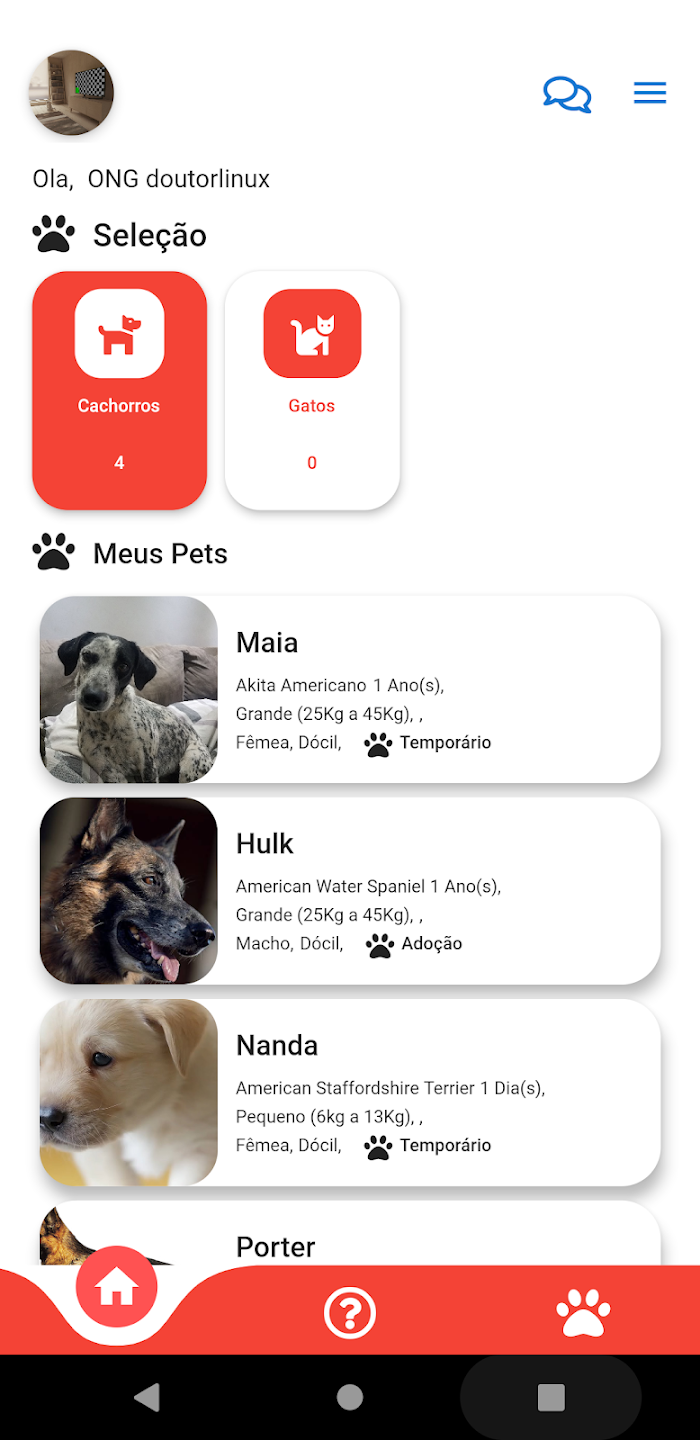
\includegraphics[width=6cm]{arquivos/Figuras/image20.png}
     \caption{Interface de aplicativo Pet Ponto}
     \label{fig:Pet Ponto}
\end{figure}
\newpage
Apesar de possuir a funcionalidade de geolocalização em seu sistema, o Pet Ponto não permite que a comunidade contribua para o rastreamento de animais perdidos por meio da geolocalização, limitando-se apenas a indicar animais para adoção com base na proximidade com o usuário. Essa diferença em relação ao MeuPetAqui torna as aplicações distintas em termos de funcionalidades oferecidas aos usuários.
\section{Arknoah}

A Arknoah é uma plataforma brasileira de rede social voltada para amantes de animais de estimação, fornecedores de produtos e serviços, bem como ONGs. De acordo com o site da plataforma \citeonline{Arknoah}, a plataforma oferece quatro perfis de usuário, cada um com funções distintas e exclusivas, estes:
\begin{itemize}
\item ARKlover é destinado aos usuários da plataforma e oferece diversas funcionalidades, como o acompanhamento dos registros de saúde do pet, o compartilhamento de fotos, vídeos e stories. Além disso, o perfil permite que o usuário dê curtidas e faça comentários em postagens e stories. O ARK ID é uma funcionalidade adicional que fornece um documento de identificação do pet que pode ser acessado por meio de um QR code. O perfil ARKlover é gratuito, mas os usuários podem optar por planos de assinatura para impulsionar a visibilidade de suas postagens, com preços que variam de R\$24,90 a R\$99,90.

\item ARKbest é voltado para comerciantes que atuam com produtos pet e permite que eles cadastrem seus negócios na plataforma gratuitamente. Os usuários podem, ainda, assinar planos mensais para impulsionar a divulgação de seus produtos na plataforma. Os preços dos planos variam de R\$24,90 a R\$99,90, dependendo da quantidade de dias de impulsionamento.

\item ARKangel é utilizado por ONGs para divulgar seus trabalhos e animais disponíveis para adoção. Assim como o ARKlover, o ARKangel é gratuito, mas os usuários podem optar por planos de assinatura para impulsionar a popularidade de suas postagens na plataforma. Os preços dos planos variam de R\$24,90 a R\$99,90.

\newpage
\item ARKpet é específico para o pet cadastrado em um perfil ARKlover. Ele contém todas as informações do animal de estimação e todas as funcionalidades do perfil ARKlover. (Figura \ref{fig:ARKNOAH}).
\end{itemize}


\begin{figure}[htb]
     \centering
     \FonteFig{ARKNOAH/Google Play}
     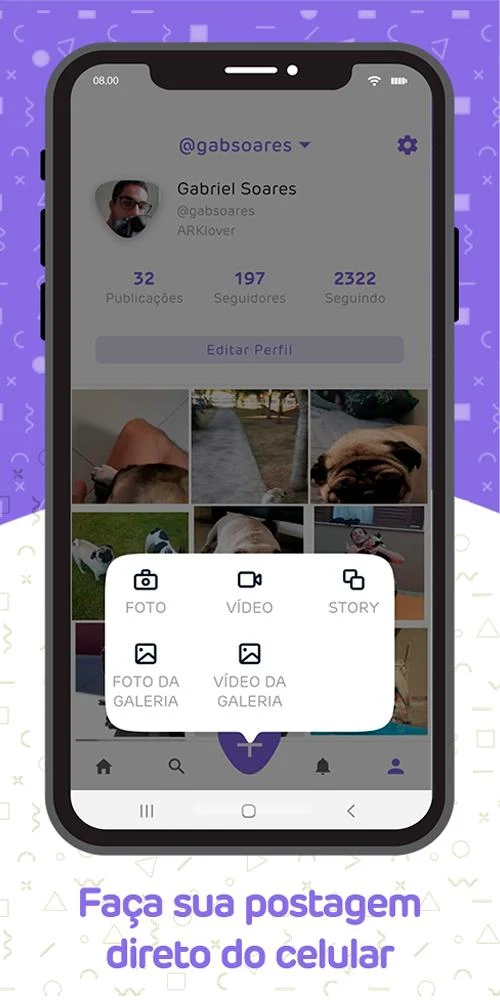
\includegraphics[width=6cm]{arquivos/Figuras/image23.png}
     \caption{Interface de aplicativo ARKNOAH - Criação de Posts}
     \label{fig:ARKNOAH}
\end{figure}
Assim como o Flockr, o Arknoah é uma aplicação que possui funcionalidades pagas, o que pode desencorajar alguns usuários em potencial. Além disso, uma diferença significativa em relação ao MeuPetAqui é a ausência de serviços de rastreamento de animais perdidos na plataforma do Arknoah. Isso pode ser um fator a ser considerado por usuários que valorizam a possibilidade de localizar seus animais de estimação em caso de perda.

\newpage
\section{Appegada}
Em seu site, \citeonline{APPEGADA}, o sistema Appegada, tem as suas funcionalidades descritas, sendo este um marketplace focado em produtos para animais, que também conta com funcionalidades para os donos de pets, sendo estas:
\begin{itemize}
\item Localização de clínicas veterinárias e petshops.
\item Plano de Saúde do Pet.
\item Criar postagens do pet e acompanhar postagens de outros tutores.
\item Catálogo de pets perdidos ou encontrados.
\item Catálogo de pets para adoção.
\end{itemize}
Demonstração da aplicação na APP Store na \ref{fig:Appegada}.

\begin{figure}[htb]
     \centering
     \FonteFig{Appegada/App Store}
     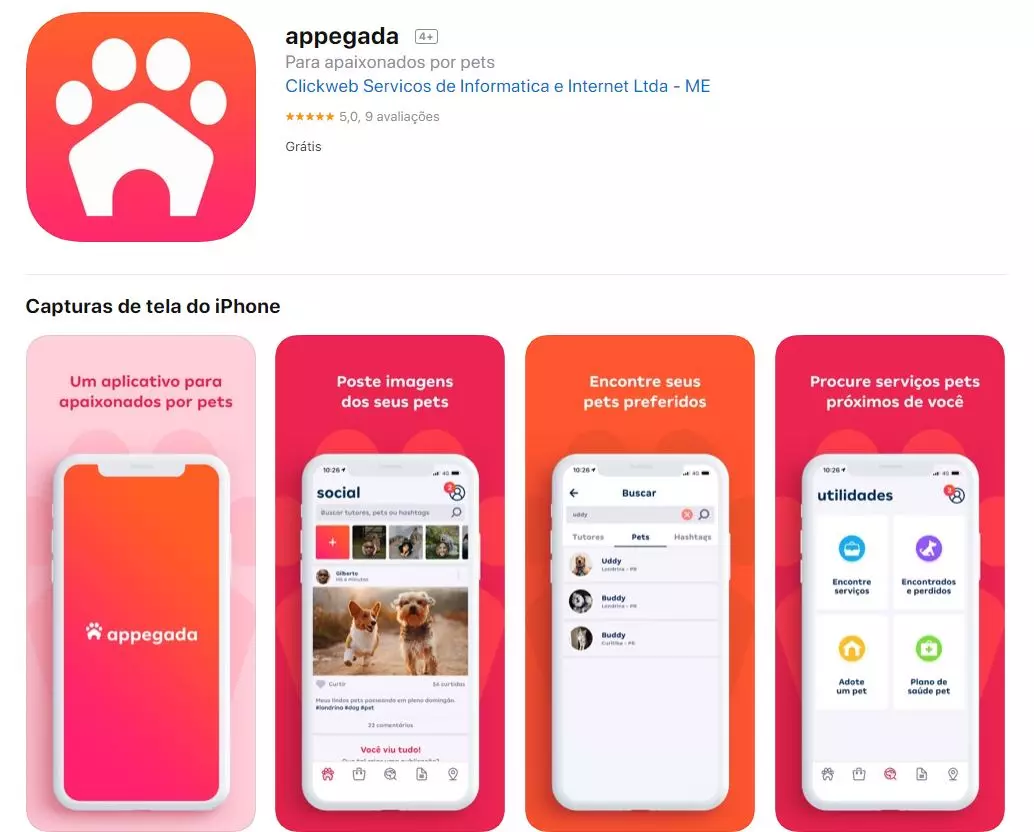
\includegraphics[width=12cm]{arquivos/Figuras/image8.png}
     \caption{Interface de aplicativo Appegada}
     \label{fig:Appegada}
\end{figure}

O Appegada não oferece um serviço de rastreamento de pets perdidos, o que pode ser considerado uma desvantagem em comparação com o MeuPetAqui. Essa importante funcionalidade pode influenciar na escolha entre as duas plataformas.

\newpage
\section{PUPZ}
Com base em pesquisas ao site da \citeonline{PUPZ}, pode-se observar que a plataforma é voltada ao rastreamento de pets. O sistema da PUPZ permite o rastreamento de pets por meio de coleiras equipadas com chips NFC\footnote{NFC - Near Field Communication, é uma tecnologia de comunicação sem fio que permite a troca de informações entre dispositivos que estejam próximos um do outro}, que são comercializadas dentro da própria plataforma. Com essa funcionalidade, o usuário consegue acompanhar a posição do pet por meio de um mapa que exibe a localização da coleira. Além do rastreamento por meio do chip, a plataforma permite a comparação entre o pet encontrado ou perdido e os pets cadastrados no sistema, utilizando biometria facial do animal por meio do mapeamento de padrões presentes na face do pet.

De acordo com Fabbro, desenvolvedor do sistema, a precisão do reconhecimento facial possui um índice de assertividade/acuracidade acima de 90\%, sendo capaz de identificar cães e gatos \cite{Fabbro}. (Figura \ref{fig:PUPZ}).

\begin{figure}[htb]
     \centering
     \FonteFig{PUPZ}
     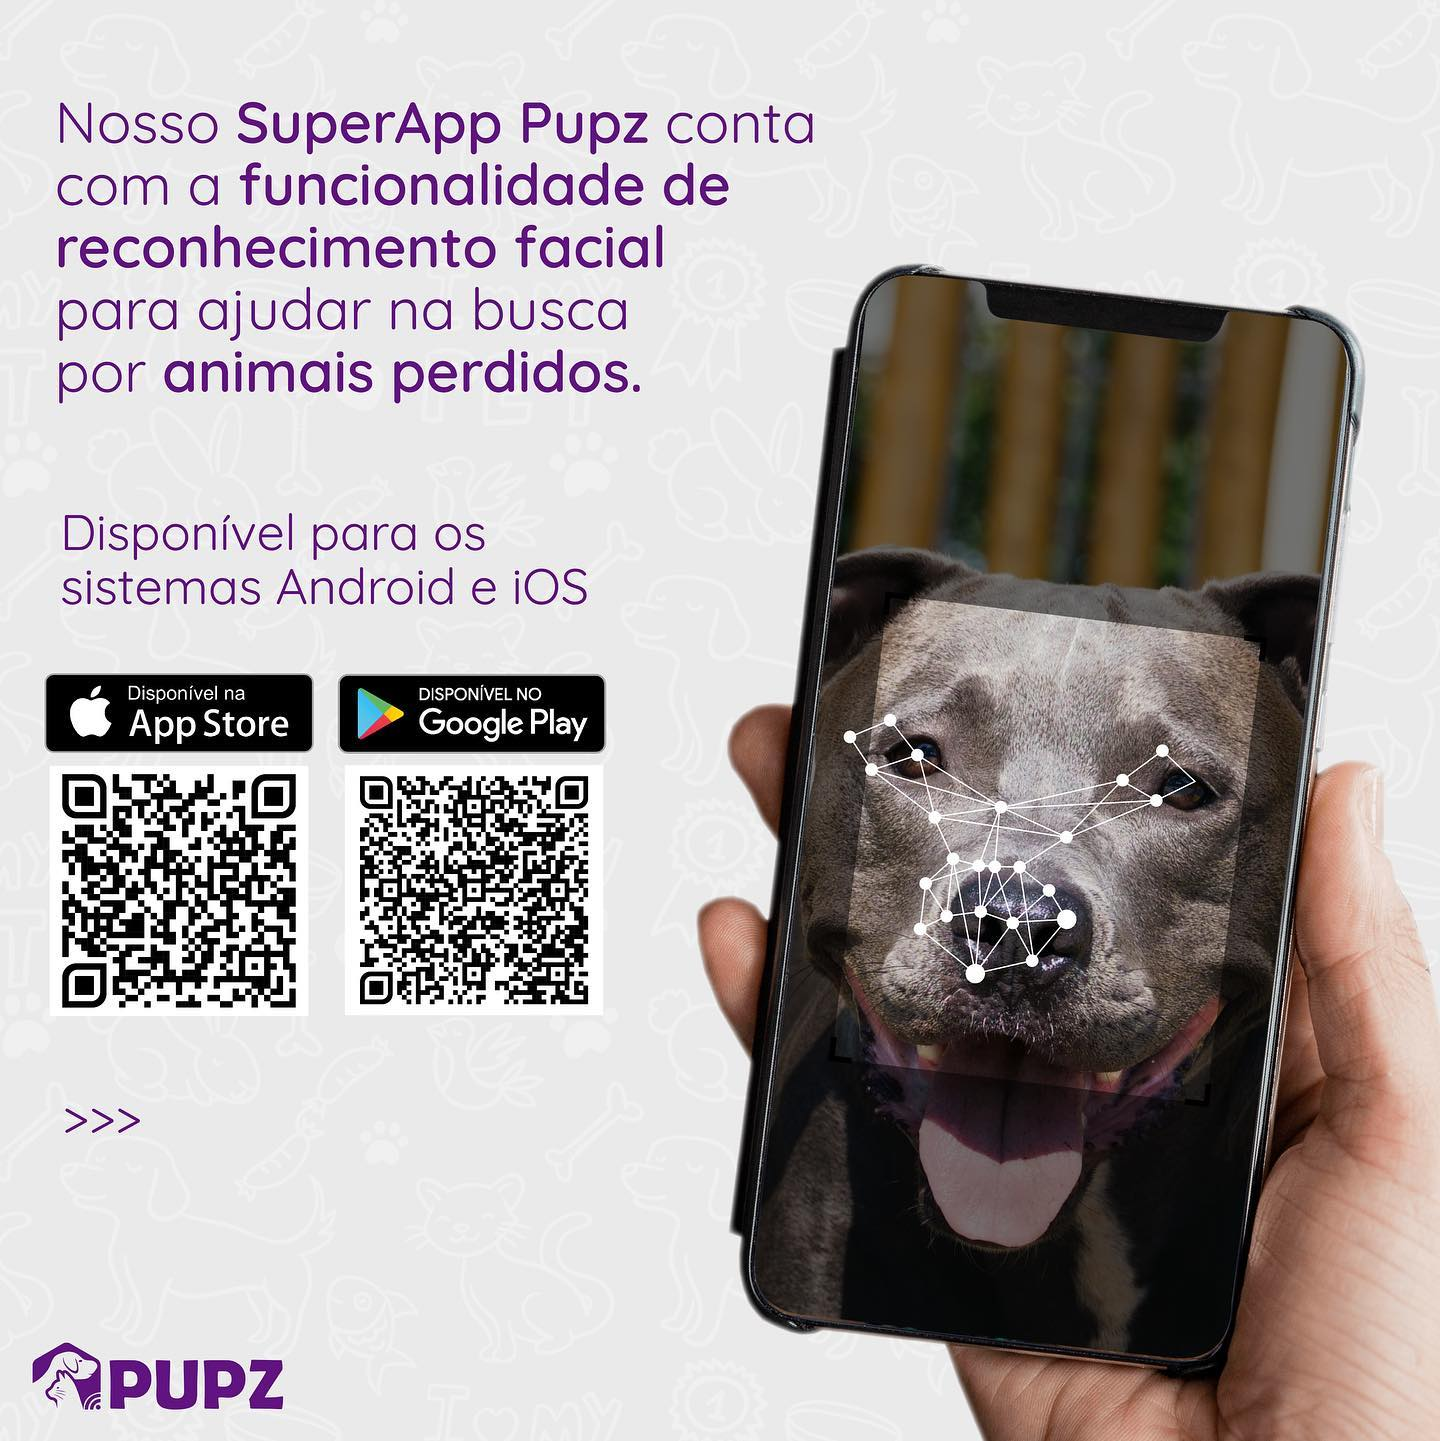
\includegraphics[width=10cm]{arquivos/Figuras/image15.jpg}
     \caption{Campanha publicitária PUPZ}
     \label{fig:PUPZ}
\end{figure}

\newpage
O PUPZ é um serviço que oferece rastreamento de pets, o que o diferencia do MeuPetAqui, que é uma rede social com várias funcionalidades, incluindo o rastreamento. É importante ressaltar que o rastreamento no PUPZ requer a aquisição de uma coleira específica fornecida pela empresa responsável pela aplicação. A necessidade de arcar com os custos da coleira é outro ponto que diferencia o PUPZ, já que o MeuPetAqui oferece essa funcionalidade de forma gratuita. Essa diferença pode ser um fator a ser considerado pelos usuários ao escolher entre as duas plataformas.
\section{Izoo }
Ao acessar o site \citeonline{IZOO}, é possível constatar que a plataforma se trata de uma rede social para donos de animais criarem perfis para seus pets e interagirem com outros usuários. Além das funções comuns encontradas em redes sociais, como a criação, comentários e curtidas de posts, a plataforma também oferece o serviço de identificação de pets cadastrados por meio de um código exclusivo fornecido quando se adquire um pingente comercializado em seu site. Caso o pet desse usuário se perca, quem o encontrar poderá buscar informações do pet e descobrir quem é seu tutor, bastando informar ao sistema o código presente no pingente. A plataforma também conta com funcionalidades como:
\begin{itemize}
\item Caderneta virtual (vacinas, medicamentos, eventos).
\item Marketplace de produtos relacionados à animais de estimação.
\item Divulgação de pets perdidos ou encontrados ou disponíveis para adoção.
\end{itemize}
Assim como outros serviços mencionados, o IZOO é uma rede social que não oferece a funcionalidade de rastreamento de pets perdidos. Essa falta de recurso se torna uma grande desvantagem em comparação com o MeuPetAqui, que disponibiliza essa importante ferramenta para auxiliar na localização e recuperação de animais perdidos.

\section{AlertPet}
No site \citeonline{ALERTPET}, pode-se observar que a aplicação se divide em duas ações voltadas ao bem-estar animal. A primeira ação é a divulgação de animais perdidos ou disponíveis para adoção, que são exibidos no próprio site. Já a segunda ação consiste na assinatura do serviço de impulsionamento de postagens. O usuário cria uma postagem informando a situação, como a perda de seu pet, por exemplo, e o sistema impulsiona esse post nas redes sociais Facebook e Instagram. Os planos de assinatura variam de acordo com a quantidade de destinatários e distância de abrangência, com valores que oscilam entre R\$97 e R\$493.

O AlertPet é um serviço dedicado à divulgação de pets perdidos ou disponíveis para adoção, diferentemente do MeuPetAqui que oferece funcionalidades de uma rede social. Além disso, uma distinção significativa entre as plataformas é que o AlertPet requer pagamento pelos serviços de rastreamento, o que pode desencorajar a participação de uma parcela importante de potenciais usuários. Essas diferenças ressaltam a abordagem distinta entre o AlertPet e o MeuPetAqui, tanto em termos de funcionalidades oferecidas quanto na disponibilidade de recursos gratuitos.

\newpage
\section{Comparação entre plataformas}

\begin{table}[htb]
    \centering
    \footnotesize
    \caption{Características e funcionalidades presentes nas plataformas}
    \begin{tabular}{|p{2.2cm}|c|c|c|c|c|c|c|c|c|}
        \hline
        \textbf{Função} & \textbf{Flockr} & \textbf{Pet} & \textbf{Arknoah} & \textbf{Appegada} & \textbf{PUPZ} & \textbf{IZZO} & \textbf{AlertPet} & \textbf{MeuPetAqui}\\
        \hline
        Rede 
        Social & \faCheck & - & \faCheck & \faCheck & - & \faCheck & - & \faCheck\\
        \hline
        Encontrar \mbox{Pet Perdido} & \faTimes & \faCheck & \faTimes & \faCheck & \faCheck & \faCheck & \faCheck & \faCheck\\
        \hline
        Encontrar \mbox{Tutor} & \faTimes & \faCheck & \faTimes & \faCheck & \faCheck & \faCheck & \faTimes & \faCheck\\
        \hline
        Pets Para Adoção & \faTimes & \faCheck & \faCheck & \faCheck & \faTimes & \faCheck & \faTimes & \faCheck\\
        \hline
        Contribuir Com ONGs & \faTimes & \faCheck & \faCheck & \faCheck & \faTimes & \faCheck & \faTimes & \faCheck\\
        \hline
        Serviços \mbox{Gratuitos} & \faCheck & \faCheck & \faCheck & \faCheck & \faCheck & \faCheck & \faTimes & \faCheck\\
        \hline
        Serviços \mbox{Pagos} & \faCheck & \faTimes & \faCheck & \faCheck & \faTimes & \faTimes & \faCheck & \faTimes\\
        \hline
        Plano De Saúde & \faCheck & \faTimes & \faTimes & \faCheck & \faTimes & \faTimes & \faTimes & \faTimes\\
        \hline
        Marketplace & \faTimes & \faTimes & \faCheck & \faCheck & \faCheck & \faCheck & \faTimes & \faTimes\\
        \hline
        Rastreio Com Chip & \faTimes & \faTimes & \faTimes & \faTimes & \faCheck & \faTimes & \faTimes & \faTimes\\
        \hline
        Rastreio Por Interação & \faTimes & \faCheck & \faTimes & \faCheck & \faCheck & \faCheck & \faCheck & \faCheck\\
        \hline
        Mapa de \mbox{Localização} & \faTimes & \faTimes & \faTimes & \faTimes & \faCheck & \faTimes & \faTimes & \faCheck\\
        \hline
        Perfil Para Pet & \faCheck & \faTimes & \faCheck & \faTimes & \faTimes & \faCheck & \faTimes & \faCheck\\
        \hline
        Carteira de Identificação & \faTimes & \faTimes & \faCheck & \faTimes & \faTimes & \faTimes & \faTimes & \faCheck\\
        \hline
        Acompanhar Medicações & \faCheck & \faTimes & \faCheck & \faTimes & \faTimes & \faCheck & \faTimes & \faCheck\\
        \hline
    \end{tabular}    
    \caption*{\footnotesize  Fonte: Elaborado pelo autor}
    \label{tab:Plataformas}
\end{table}

Outro aspecto relevante a ser considerado é a barreira geográfica apresentada pelas aplicações mencionadas. Esses serviços são regionalizados, o que significa que sua divulgação e utilização são limitadas a determinadas regiões, resultando em pouca ou nenhuma familiaridade com o público de Vitória da Conquista, que é o principal alvo do MeuPetAqui. Isso destaca a vantagem competitiva do MeuPetAqui, que tem como foco atender especificamente essa população e oferecer uma solução adaptada às suas necessidades locais.
%%%%%%%%%%%%%%%%%%%%%%%%%%%%%
% \section{Levantamento do Estado da Arte}

% É no capítulo de Referencial Teórico que se levanta o \textbf{ESTADO DA ARTE}, que mostra o que já se tem estudado e o que se tem feito no tema abordado no seu trabalho:
    
% \begin{description}
%     \item [ESTADO DA ARTE:] O Estado da Arte é uma referência ao estado atual de conhecimento sobre um determinado tópico que está sendo objeto de análise ou estudo. De forma geral, o estado da arte representa o nível mais alto de um processo de desenvolvimento, seja de um aparelho, de uma técnica ou de uma área científica, alcançado até um determinado momento. 
% \end{description}



% %%%%%%%%%%%%%%%%%%%%%%%%%%%%
% \section{Levantamento do Estado da Técnica}

% Caso o seu trabalho venha a citar alguma {\bf patente} ou algum trabalho que esteja protegido por {propriedade intelectual}, você deve levantar o \textbf{ESTADO DA TÉCNICA}, as \textbf{INVENÇÕES} e \textbf{MODELOS DE UTILIDADE}.

% \begin{description}
%     \item [ESTADO DA TÉCNICA:] O Estado da técnica é um termo usado na propriedade industrial e compreende tudo aquilo que foi tornado acessível ao público antes da data de depósito do pedido de patente, por descrição escrita ou oral, por uso ou qualquer outro meio, no Brasil ou no exterior. Isso significa que a invenção e o modelo de utilidade são considerados novos somente quando não estão compreendidos no estado da técnica.
%     Logo, se uma invenção ou modelo de utilidade já foi divulgado ao público antes do depósito do pedido de patente, ele é considerado parte do estado da técnica e não é mais considerado novo.
    
%     \item[INVENÇÃO:] A Invenção é uma criação industrial que pode ser explorada economicamente e que atende a quatro requisitos previstos na lei de propriedade industrial (Lei nº 9.279/1996): novidade, atividade inventiva e aplicação industrial. Isso significa que para ser considerada uma invenção e ser patenteada, a criação deve ser nova, não óbvia para um técnico no assunto, ter aplicação industrial e não estar impedida por outras leis ou regulamentos.
    
%     \item[MODELO DE UTILIDADE:] O Modelo de Utilidade é uma modalidade de patente que se destina a proteger inovações com menor carga inventiva, normalmente resultantes da atividade do operário ou artífice1. É o objeto de uso prático suscetível de aplicação industrial, como novo formato de que resulta melhores condições de uso ou fabricação.
% \end{description}

% %%%%%%%%%%%%%%%%%%%%%%%%%%%%%%

% \section{Não confunda Introdução e  Referencial Teórico}

% É muito frequente a confusão do que deve ser escrito no capítulo de {\bf Introdução} e o que deve ser escrito no capítulo de {\bf Referencial Teórico}.

% A principal diferença é que no {\bf capítulo de Introdução} você irá mostrar ao leitor do que se trata o seu trabalho e o que o leitor irá encontrar ao ler o seu texto.

% Já no {\bf capítulo de Referencial Teórico}, você irá mostrar ao leitor que você conhece o que outros autores já fizeram no mesmo tema que você está trabalhando, e que o seu trabalho é no que o seu trabalho é diferente ou complementa outros trabalhos de outros autores.

% %%%%%%%%%%%%%%%%%%%%%%%%%%%%

% \section{Como realizar citações automáticas de Referências}

% A forma correta de se referenciar em \LaTeX é utilizando a ferramenta {\bf BibTeX}.

% Uma ótima forma de utilizar o {\bf BibTeX} é criando uma biblioteca {\bf *.bib} e adicionar todas as nossas referências dentro dela.

% %%%%%%%%%%%%%%%%%%%%%%%%%%%%%%

% \subsection{Utilizando o BibTeX}

% Para este template de PFC e Relatório, foi criada uma biblioteca exemplo com o nome {\bf bib\_pfc.bib}, que você pode encontrar na figura~\ref{fig:bib_pfc}. 

% Veja na figura~\ref{fig:bib_pfc} o formato do código \LaTeX~ do arquivo {\bf bib\_pfc.bib}.

% \begin{figure}[htb]
%     \centering    
%     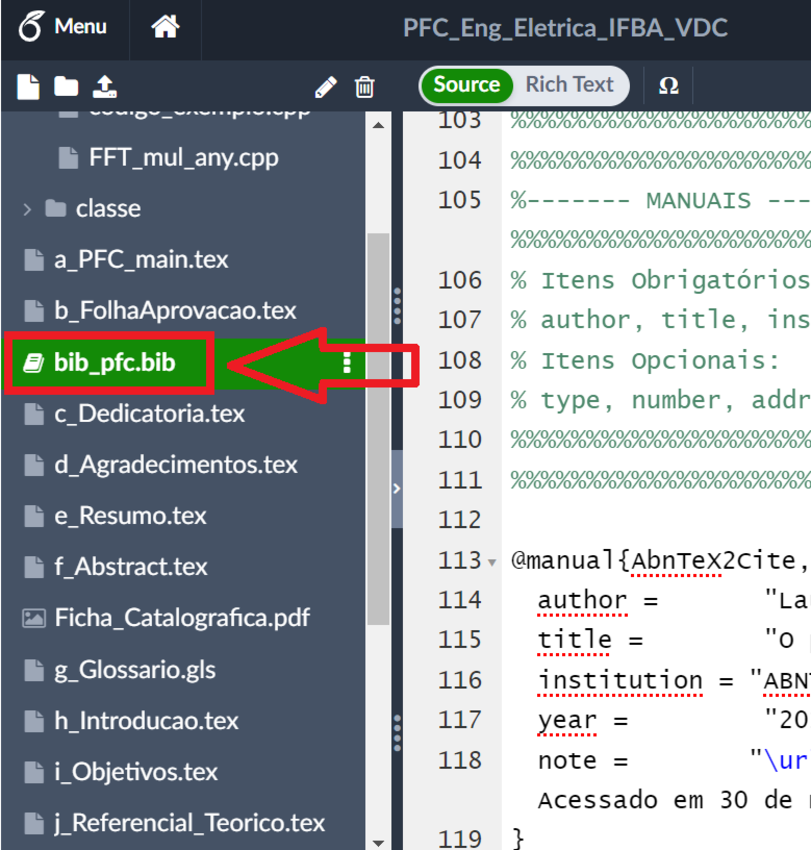
\includegraphics[width=9cm]{arquivos/arqcls/Fig_bib_pfc.pdf}
%     \FonteFig{Próprio Autor}
%     \caption{Localização da biblioteca  {\bf bib\_pfc.bib} criada para este template no LaTeX-Overleaf}    
%     \label{fig:bib_pfc}
% \end{figure}

% \begin{CaixaVerde}
%     Acrescente todas as suas referências a serem utilizadas no seu trabalho aqui neste arquivo {\bf bib\_pfc.bib}
% \end{CaixaVerde}

% Um exemplo de formatação de citação do artigo~\cite{CHANG}, também pode ser citado com o nome do autor desta forma~\citeonline{CHANG}. Esta citação no arquivo {\bf bib\_pfc.bib} está mostrado no código~\ref{cod:BibTeX}.  

% \begin{Codigo}[language=tex, 
%     caption=Exemplo de alimentação do arquivo {bib\_pfc.bib}, 
%     label=cod:BibTeX]
% @article{CHIN,
%   author =  "Chin Chang and Gert W. Bruning",
%   title =   "Analysis of the Self-Oscillating Series Resonant 
%              Inverter for Electronic Ballasts",
%   journal = "IEE TRANSACTIONS ON POWER ELECTRONICS",
%   year =    "1999",
%   volume =  "14"  
% }
% \end{Codigo}

% \pagebreak
% No arquivo {\bf bib\_pfc.bib} estão as orientações de como acrescentar suas referências, contendo os itens obrigatórios e opcionais. As referências suportadas mais utilizadas são mostradas na tabela~\ref{tab:Tipos_Ref}: 
    
% \begin{table}[htb]
%     \centering
%     \caption{Principais tipos de referências mais utilizadas}
%     \begin{tabular}{ll}
%         \toprule
%         Article         & = Artigos \\
%         Book            & = Livros \\
%         Manual          & = Manuais \\
%         mastersthesis   & = Dissertações de Mestrado \\
%         phdthesis       & = Teses de Doutorado \\
%         techreport      & = Normas Técnicas \\
%         unpublished     & = Citações da Internet\\
%         \bottomrule
%     \end{tabular}        
%     \label{tab:Tipos_Ref}
% \end{table}
    
%  Para  mais tipos de referências além das citadas na tabela~\ref{tab:Tipos_Ref}, consulte o site da ferramenta BibTeX: \url{https://en.wikipedia.org/wiki/BibTeX}. 
% Aqui neste modelo (template) está configurado a ferramenta {\bf AbnTeX2Cite} \cite{AbnTeX2Cite} que segue a norma brasileira ~\citeonline{NBR6023_Referencias}.

% %%%%%%%%%%%%%%%%%%%%%%%%%%%%

% \subsection{Citações de Referências com os comandos: cite e  citeonline}

% Os comandos de citação mais utilizados são: \verb|\cite{}| e  \verb|\citeonline{}|. Existem outros formatos específicos que podem ser consultados no manual da ferramenta {\bf AbnTex2Cite} \cite{AbnTeX2Cite}.

% Note que após realizar a citação no texto o ~\LaTeX~ já cria automaticamente as referências no capítulo de referências formatado de acordo com a norma~\citeonline{NBR6023_Referencias}, conforme mostrado no capítulo de Referências na página~\pageref{cap:RefBib}.


% O comando \verb|\cite{}| cita a referência no texto da seguinte forma: \cite{GeraHarm_CONNEPI_Elvio_Iuri}, já o comando \verb|\citeonline{}| cita uma referência chamando o autor no texto como por exemplo: "De acordo com \citeonline{phd_Dertien} a robótica\ldots"

%  Para mais detalhes de como utilizar a ferramenta de citações automáticas e se precisar de mais comandos específicos para citações, de acordo com a \citeonline{NBR6023_Referencias}, consulte o documento {\bf AbnTex2Cite}:

%  \url{http://tug.ctan.org/macros/latex/contrib/abntex2/doc/abntex2cite.pdf}


% \section{Realizar as Referências buscando em repositórios e bases de dados indexados}

% As referências devem ser citadas ao longo do texto e devem conter livros, normas, manuais e artigos que foram utilizados como literatura para o projeto.
    
% Evitar referências a apostilas e sites de internet com conteúdo não revisado, como blogs e wikipedia, pois como não estão sujeitos a revisão, podem conter conteúdo errado ou não regulamentado.

% Para que a referência que você irá citar tenha relevância, ela precisa ter vindo de alguma fonte que foi revisada por profissionais especializados na área. Os livros, dissertações de mestrado, teses de doutorado, artigos de revistas e conferências científicas, passam por correções e avaliações por pares, validando o conteúdo científico.  
    
% Procure selecionar sites de internet que são confiáveis e revisados, tais como sites de:

% \begin{enumerate}
%     \item Revistas científicas indexadas;
%     \item Conferências e congressos;
%     \item Teses, Dissertações, Monografias;
%     \item Patentes;
%     \item Repositórios Científicos;
%     \item Fabricantes;
%     \item Manuais de utilização;
%     \item Normas Técnicas (ABNT, IEEE, IEC, ISO\ldots);
%     \item Normas Regulamentadoras (NR);  
%     \item Legislação;
%     \item Universidades;
% \end{enumerate}

% Seguem alguns exemplos de fontes confiáveis:

% \begin{itemize}
%     \item Domínio Público do MEC:\\
%     \url{http://www.dominiopublico.gov.br/};

%     \item Periódicos da Capes:\\
%     \url{http://www.periodicos.capes.gov.br/} ;

%     \item Periódicos Compendex:\\
%     \url{https://www.engineeringvillage.com/search/quick.url}

%     \item Espacenet: \\ \url{http://worldwide.espacenet.com/}

%     \item IEEE Xplore: \\
%     \url{http://ieeexplore.ieee.org/Xplore/home.jsp}%

%     \item Science Direct: \\
%     \url{https://www.sciencedirect.com/}
    
%     \item SciELO - Brasil: \\
%     \url{https://www.scielo.br/}

%     \item Google Acadêmico: \\
%     \url{https://scholar.google.com.br/?hl=pt}

%     \item Elsevier: \\
%     \url{https://www.elsevier.com/pt-br}
% \end{itemize}

% Outra forma confiável é a busca em  repositórios de Teses e Dissertações de Universidades.

% Um ótimo vídeo sobre como realizar busca nas bases {\bf Science Direct} pode ser encontrado no canal ~"Descomplicando"~ do professor Henrique R. Frigeri: \url{https://youtu.be/ThcB65kcuiM}.

% %%%%%%%%%%%%%%%%%%%%%%%%%%%%

% \section{Organizador de Referências: Mendeley}

% Mendeley é uma empresa sediada em Londres, Reino Unido, que desenvolve produtos e serviços para pesquisadores acadêmicos. É conhecida principalmente por seu {\bf gerenciador de referências, usado para gerenciar, compartilhar e criar referências bibliográficas para artigos acadêmicos}.

% O Mendeley pode ser acessado em \url{https://www.mendeley.com/}, e pode ser utilizado em sua forma online ou pode ser feito o download do programa de gerenciamento de referências.

% Mendeley é um gerenciador de referências e uma rede social acadêmica que ajuda a organizar sua pesquisa, colaborar com outras pessoas on-line e descobrir as pesquisas mais recentes.

% \begin{CaixaVerde}
%     O Mendeley fornece um {\bf gerenciador de referência gratuito} que auxilia nos trabalhos acadêmicos e tem a finalidade de gerenciar arquivos eletrônicos (formato PDF), além de ajudar na normalização de citações e referências geradas automaticamente.
% \end{CaixaVerde}

% \begin{CaixaVermelha}
%     {\large O Mendeley gera automaticamente referências no formato {\bf BibTeX}.}
% \end{CaixaVermelha}

% Você pode criar uma conta gratuita e acessar sua biblioteca em qualquer lugar. Além disso, você pode gerar referências, citações e bibliografias em uma ampla variedade de estilos de revistas com apenas alguns cliques. Você também pode ler artigos em qualquer lugar com aplicativos para iOS e Android.

% Um ótimo vídeo sobre o Mendeley pode ser acessado no canal do professor Lucas Pantuza Amorim: \url{https://youtu.be/rCQhAJlW4qc}.

% %%%%%%%%%%%%%%%%%%%%%%

% \subsection{Vantagens em utilizar o gerenciador de referências Mendeley}

% Algumas vantagens em utilizar o Mendeley para gerenciar as referências de sua pesquisa:

% \begin{itemize}
%     \item Ajuda a organizar sua pesquisa e gerenciar arquivos eletrônicos (formato PDF);
%     \item Ajuda na normalização de citações e referências geradas automaticamente;
%     \item Permite acessar sua biblioteca em qualquer lugar;
%     \item Permite gerar referências, citações e bibliografias em uma ampla variedade de estilos de revistas com apenas alguns cliques;
%     \item {\bf Exporta referências no formato BibTeX};
%     \item É uma rede social acadêmica que permite colaborar com outras pessoas on-line e descobrir as pesquisas mais recentes;
%     \item Possui aplicativos para iOS e Android para ler artigos em qualquer lugar;
%     \item O Mendeley organiza todos os seus artigos, documentos, etc, ajuda a localizar o texto que você precisa, e exporta a referência no formato que você precisar (BibTeX por exemplo);
%     \item Ao invés de você guardar todos as suas dezenas de  artigos e referências em uma pasta no computador e depois não saber mais qual deles tem o texto que você precisa, você irá guardar tudo no Mendeley e quando precisar, o Mendeley te ajudará a encontrar o que precisar.
%     \item Com o Mendeley você poderá fazer anotações, grifar, registrar e comentar suas referências de forma a conseguir encontrar o que precisa na hora de escrever seu trabalho definitivo;
%     \item O Mendeley te ajuda a criar o capítulo de Referencial Teórico com levantamento bibliográfico;
% \end{itemize}

% \begin{CaixaVerde}
%     Imagine que você já leu dezenas de artigos, manuais, documentos, teses e dissertações no tema de seu projeto, porém na hora de escrever o capítulo de Referencial Teórico {\bf você não lembra mais} qual foi o artigo que está um determinado assunto que você precisa citar. {\bf Pode ter certeza que isso vai acontecer,} e o Mendeley foi feito para organizar suas referências para que você consiga encontrar tudo o que precisa.
% \end{CaixaVerde}

